%----------------------------------------------------------------------------
%bb defines the bounding box for the pdf
%viewport defines the area of the pdf used
%in sidewaysfigure the last entry in bb moves the caption toward/away the pic
%in sidewaysfigure the second entry in bb moves the pic toward/away the caption
%----------------------------------------------------------------------------
\begin{figure}
\scalebox{0.6}[0.6]{
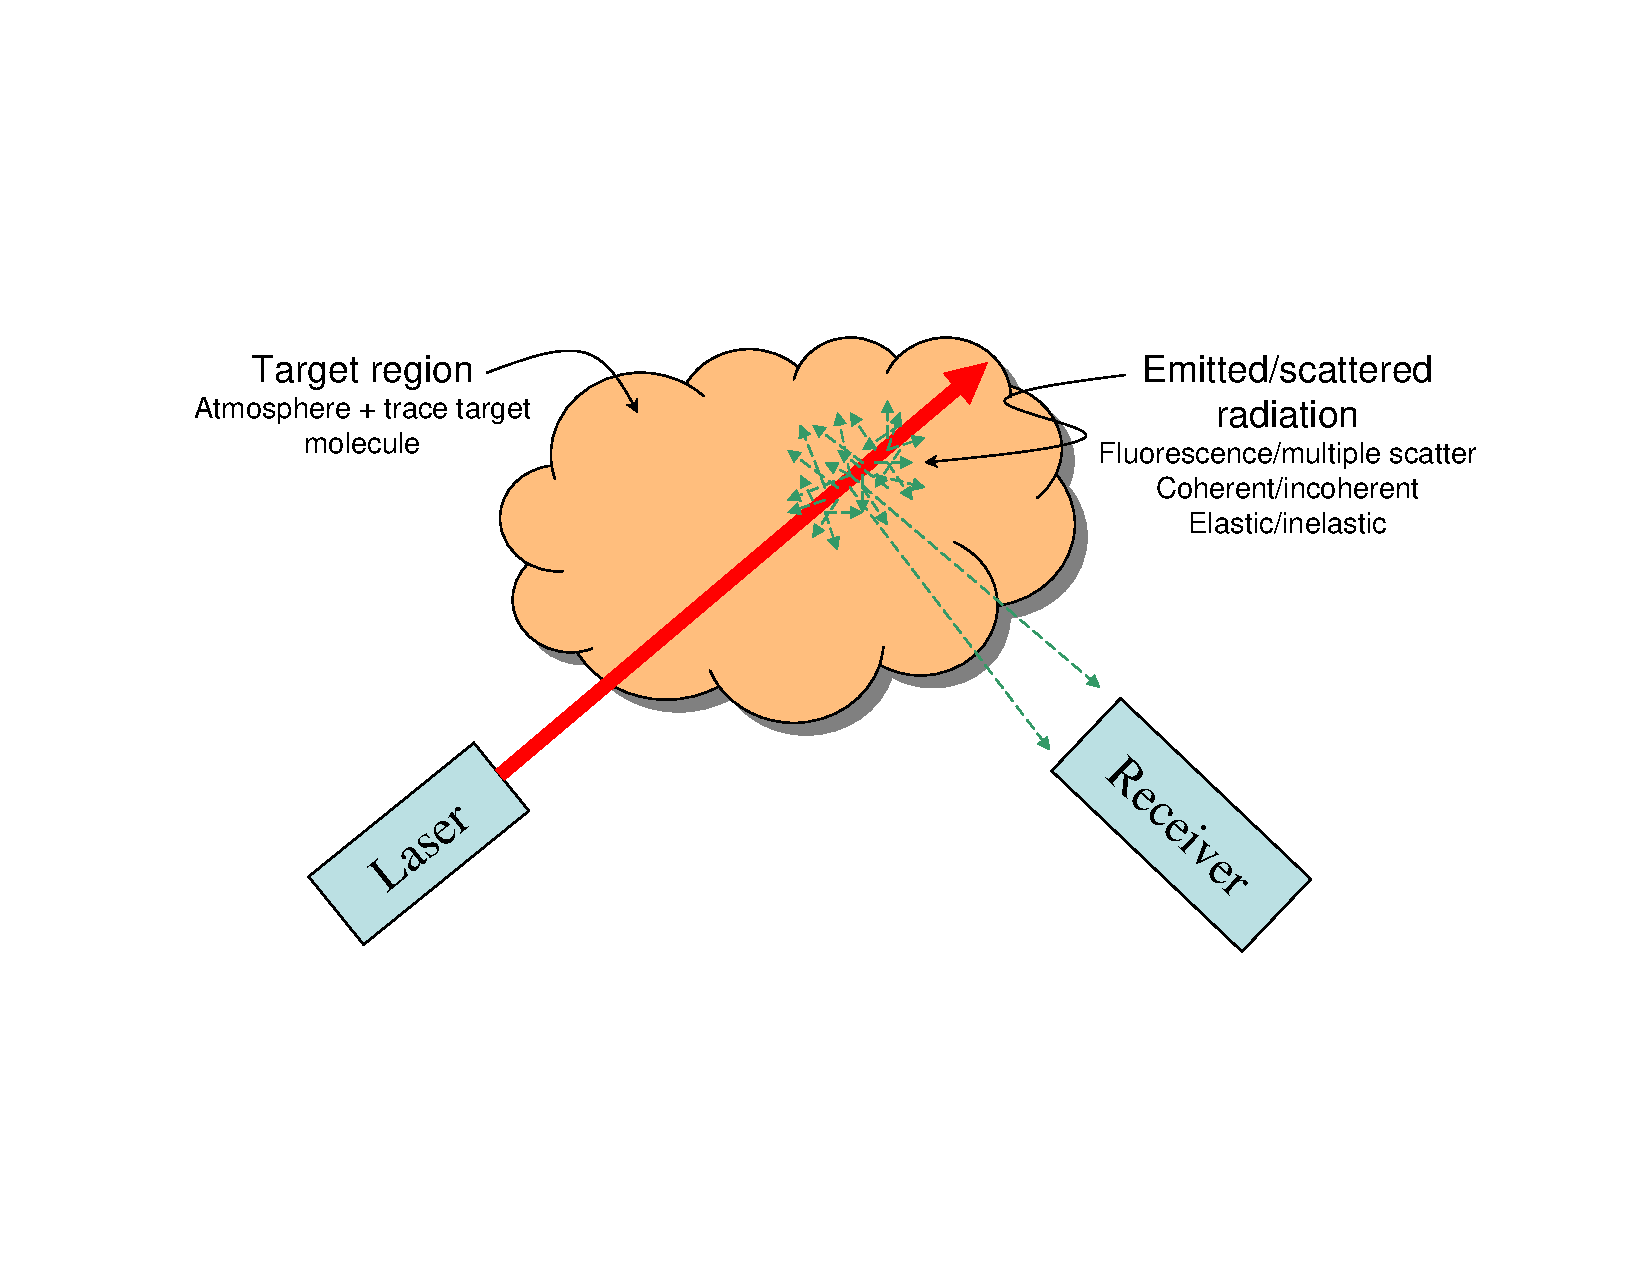
\includegraphics[bb=40 150 489 500]
{general_LIDAR/general_LIDAR.pdf}
}
\caption[General LIDAR schematic]{General remote sensing LIDAR schematic. A laser beam is used to excite a region of atmosphere while a receiver (telescope) collects the resulting emitted/scattered radiation. The spectral and temporal features of the acquired signal are used to determine the relative abundance of specific trace molecules.}
\label{general LIDAR}
\end{figure}
%----------------------------------------------------------------------------
